\chapter{Conclusions and future work}

In the preceding chapters, we discuss several research threads that I have been able to tie up into more or less complete stories during my PhD thesis.
I have been fortunate that the model I created early in my PhD thesis, described in \fref{chap:model}, has remained current and predictive for the past few years.
The model was used in some capacity in each of my publications, whether as simply an example oscillator (in \fref{chap:id} or \fref{chap:arc}), or for its biological insight (in \fref{chap:longdaysin} or \fref{chap:decay}).
Another theme throughout this thesis has been the development and subsequent implementation of various computational methods or approaches.
Specifically, the identifiability scheme discussed in \fref{chap:id} was used to make the predictions described in \fref{chap:longdaysin}, and many of the ideas described in \fref{chap:arc} were used as the motivations behind the more data-driven analysis in \fref{chap:decay}.

I am grateful to have been able to meander relatively freely from project to project, thanks in part to my Mitsubishi Chemical fellowship, and as a result each chapter largely follows from the previous work.
Despite this, there have been several research lines that, for one reason or another, I was unable to follow through with during my PhD work.
In this chapter, I describe some of those unexplored branches in the hope that a future researcher might carry on where I left off.

\section{Experimental validation of the amplitude response to metabolic stimulation}\label{sec:chida}

One of the key motivations for the development of the amplitude response curve metrics was applying the methods to metabolic perturbations.
Several studies have highlighted the importance of rhythmic food intake in maintaining high amplitude rhythms in peripheral tissues \cite{Vollmers2009, Hatori2012}.
Additionally, the importance of high-amplitude peripheral oscillations in maintaining metabolic health has been demonstrated multiple times \cite{Hatori2012, Marcheva2010}.
It is therefore likely that signals coming from rhythmic changes in metabolic state entrain peripheral oscillators and give them a temporary boost in amplitude.

In particular, we were motivated by results from Yamajuku {\itshape et al.,}, 2012, which shows that a temporary dose of insulin not only changes the phase of cultured hepatocytes, but also appears to have an effect on the amplitude of the oscillations as well (\fref{fig:yamajuku}).
This effect, while not described in the original paper, seems to be phase-dependent: insulin delivered at late times (T12-20) seems to have a small to negative effect on the amplitude, while that delivered at early times (T0-T8) has a positive effect on the amplitude.
This type of behavior would be expected if insulin indeed conveyed a ``fed'' state to the circadian oscillator, as amplitudes would only be boosted when meals arrived at the proper phase.

\begin{figure}[tbp]
  \centering
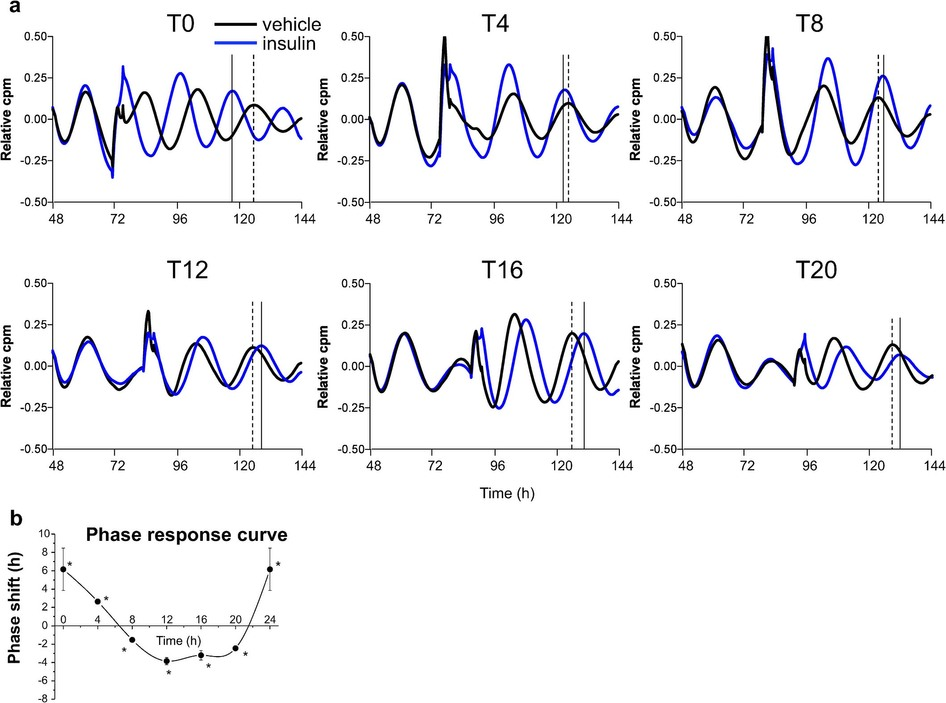
\includegraphics[width=\textwidth]{chap7/figures/yamajuku_arc.jpg}
\titlecaption{Effect on temporary insulin dosages on hepatocyte circadian gene expression}{The introduction and subsequent washing out of insulin in cultured hepatocytes leads to a phase-response curve (B), but perhaps more interestingly also seems to have an effect on the amplitude of circadian oscillations. Figure taken from \cite{Yamajuku2012}.}
  \label{fig:yamajuku}
\end{figure}

Ultimately, however, the data presented in \cite{Yamajuku2012} did not prove to be sufficient for a complete analysis.
In particular, we noted that the amplitude response due to the application of the vehicle (comparing black lines before and after the pulse, \fref{fig:yamajuku}) seems to be as significant as the amplitude change due to the application of insulin.
This is not surprising, as peripheral oscillators as acutely sensitive to changes in temperature and culture medium, which is often enough to resynchronize the population of oscillators.

We therefore sought to re-create these experiments in collaboration with Andrew Liu and Chidambaram Ramanathan at the University of Memphis.
We also hoped that by knocking out different components of the signal transduction pathway between insulin and the core clock, we might be able to elucidate a mechanism by which the amplitude response curves were occurring.

\subsection{Metabolic-circadian connections}
The literature on signalling networks connecting metabolic and circadian regulators is very dense.
Additionally, the signalling network changes over time, since many key metabolic regulators are expressed in a circadian manner.
For example energy sensors Akt and AMPK are up- or down-regulated depending on the energy and redox state of the cell \cite{Naimi2010}.
Akt, which is also a direct target of insulin \cite{Luni2011}, is known to regulate mTOR \cite{Hahn-Windgassen2005}, which is in turn known to regulate the light-mediated transcription of {\itshape Per} in the SCN \cite{Cao2010}.
Some of the key connections between insulin and core clock species are highlighted in \fref{fig:connections}

\begin{figure}[tbp]
  \centering
  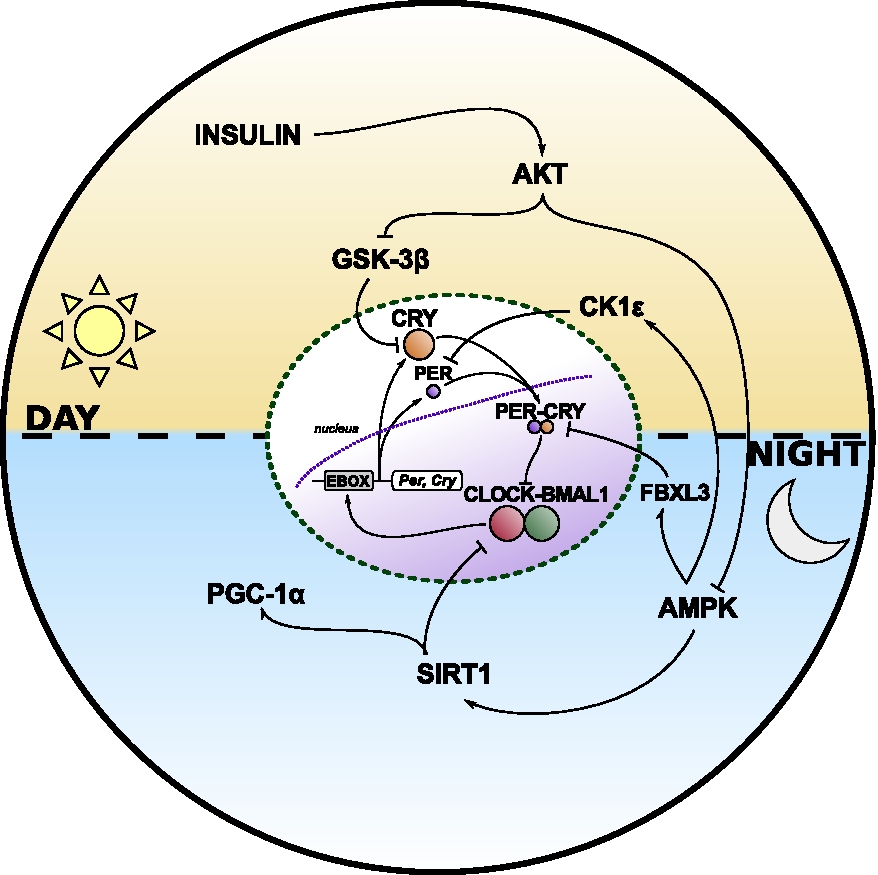
\includegraphics[width=0.7\textwidth]{chap7/figures/metabolic_connections.pdf}
  \titlecaption{Known connections between insulin and circadian rhythms}{A key step in determining potential mechanisms for the amplitude effect of insulin stimulation on circadian rhythms will be to map major signalling pathways which may be responsible for conveying information on metabolic state to the clock. Some of the connections are shown here, many of which could be independently stimulated via small molecule action.}
  \label{fig:connections}
\end{figure}

Many posttranslational regulators are also means by which cellular energy state affects circadian rhythms.
AMPK is known to affect the posttranslational regulator FBXL3, a regulator of CRY stability identified as the main target of KL001 \cite{Lamia2009}.
Additionally, AMPK has been shown to affect the activity of CKI$\delta/\epsilon$ \cite{Lee2013}, modulators of PER phosphorylation identified as main targets of longdaysin.

Since many of the targets of insulin could be independently stimulated via small molecule activators, a follow up experiment might be to directly test the time-dependent effect of small molecule modulators on circadian amplitudes.
A summary of possible small molecule modulators and pathways by which they might affect the core clock is shown in \fref{fig:small-molecule}

\begin{figure}[tbp]
  \centering
  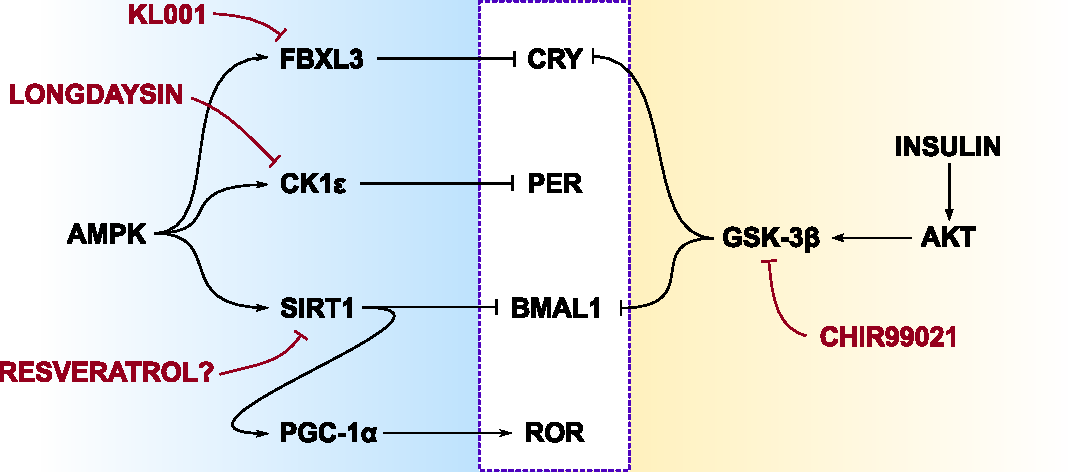
\includegraphics[width=0.8\textwidth]{chap7/figures/connectivity.pdf}
  \titlecaption{Potential small molecule candidates}{Several small molecules are known to modulate intermediate species in the insulin to core clock pathway. The phase-dependent effect of these small molecules could be independently tested in order to validate experiments using insulin.}
  \label{fig:small-molecule}
\end{figure}

\subsection{Continuous wavelet methods}\label{sec:cwt}

Several methods could be used to determine changes in amplitude or phase from experimental data.
One of method for understanding nonstationary sinusoidal signals is the continuous wavelet transform (CWT) \cite{Torrence1998}, which maps the correlation between a wavelet function and the data at a variety of scales (periods) and times.
The resulting CWT is useful for visualizing changes in phase or amplitude, as shown in \fref{fig:cwt}.
Such a tool could be used to compare the phase-dependent changes in phase and amplitude following insulin or small molecule application under a variety of conditions.

\begin{figure}[tbp]
  \centering
  \begin{subfigure}{0.475\textwidth}
    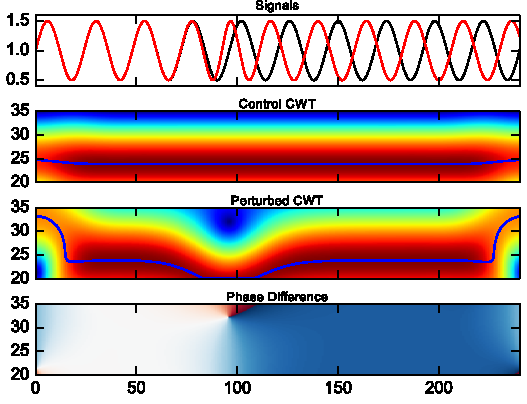
\includegraphics[width=\textwidth]{chap7/figures/phase.pdf}
    \caption{Phase Change}
  \end{subfigure}
  \begin{subfigure}{0.475\textwidth}
    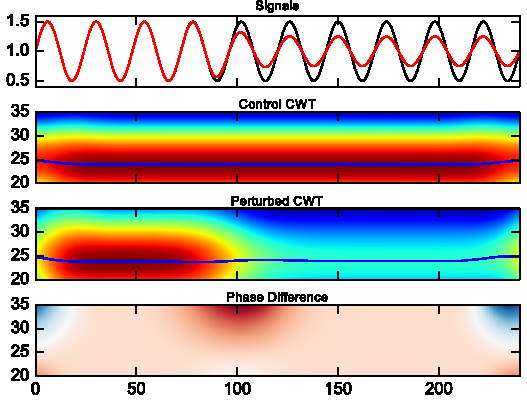
\includegraphics[width=\textwidth]{chap7/figures/amp.pdf}
    \caption{Amplitude Change}
  \end{subfigure}
  \titlecaption{Application of the continuous wavelet data to example data}{The continuous wavelet transform can be used to visualize variations in period, amplitude, or phase of a sinusoidal signal. In {\bfseries (a)}, a reference signal (black) is compared to a perturbed signal (red) with a change in phase (top). In the middle two plots, heat maps indicate the amplitude of the CWT, which remains comparable across the two signals. In the bottom plot, the difference in phase between the two signals is highlighted by a strong transition from white to blue. In {\bfseries (b)}, a change in amplitude is highlighted by a reduction in the corresponding amplitude of the CWT, with little change in phase.}
  \label{fig:cwt}
\end{figure}

\subsection{Summary}

While potentially an exciting area of research, the amplitude response characterization work has largely stalled to due experimental difficulty.
In particular, since medium changes have such a profound effect on cultured cells, it is important to perform as few disturbances as possible during the incubation period.
Unlike with studies using light as a temporary perturbation, it is likely impossible to remove exogenous inputs after their application, a requirement for finding their phase-dependent effect.
Perhaps with a more cleverly designed experimental protocol, such as coupling the induction of insulin to a light-activated promoter, such an experiment would be possible to perform accurately.
Until such time, however, the amplitude response theory will likely be primarily applicable to experimental work involving light-mediated changes.

% \section{Amplitude maximization through therapeutic treatment}
% \subsection{Optimal control strategies to maximize peripheral clock amplitude}
% \subsection{Fewest treatments, combinatorial perturbations, etc.}

\section{Further extensions to the population phase response theory}\label{sec:prd}

In \fref{chap:arc}, we pull together definitions from a variety of different sub-fields to create a model of a population of noisy oscillators, each following their own limit cycle dynamics. 
In several cases, there were further analytical treatments which could have solved in greater detail, and perhaps solutions exist in the voluminous literature on phase oscillators.
Regardless, in this section, we present some unfinished derivations and thoughts on phase populations undergoing perturbations.

\subsection{Infinitesimal population PRCs and ARCs for limiting cases}
In \fref{chap:arc}, amplitude response curves at the population-level are calculated numerically by performing a change of variables of the initial probability density function $p(\theta)$ to the probability after perturbation, $\hat{p}(\theta)$.
Infinitesimal response curves at the population level can be calculated numerically.
Phase and amplitude response curves for the population level were previously defined as:
\begin{align}
  z &\coloneqq \int_0^{2\pi} e^{i\theta} p(\theta, \tilde{t}) \; d\theta \tag{\ref{eq:zbar}}\\
  \hat{z} &\coloneqq  \int_0^{2\pi} e^{i\theta} \hat{p}(\theta, \tilde{t}) \; d\theta = \int_0^{2\pi} e^{i g(\theta)} p(\theta, \tilde{t}) \; d\theta,
  \tag{\ref{eq:zhat}}\\
  \Delta \bar{\theta} &= \angle \hat{z} - \angle z \tag{\ref{eq:popphasechange}}\\
  \Delta \rho &= |\hat{z}| - |z|.
  \tag{\ref{eq:popampchange}}
\end{align}
It would be preferable if infinitesimal curves, 
\[
  \lim_{\Delta x \to 0} \frac{\Delta \bar{\theta}}{\Delta x}
\]
be calculated analytically in the differential limit, and might lead to more efficient insight into model kinetics and the relationship between the PRC and population synchrony.

As $\Delta x \to 0$, the phase transition function $g(\theta)$ can be approximated as
\[
  g(\theta) \to \theta + \frac{d\theta}{dx}\Delta x.
\]
While its unlikely that the infinitesimal PRC and ARC could be calculated for an arbitrary $p(\theta)$, it may be possible to calculate them for the limiting cases in which the oscillators were perfectly synchronized, $p(\theta) \to \delta(\theta - \mu)$, or perfectly disperse, $p(\theta) \to {\cal U}$.

Starting first with the case where $p(\theta) \to \delta(\theta - \mu)$, we can find $\hat{z}$ directly:
\[
  \hat{z} =  \int_0^{2\pi} e^{i g(\theta)} \delta(\theta - \mu) \; d\theta = e^{i g(\mu)} = e^{i(\mu + \left.\frac{d\theta}{dx}\right|_\mu \Delta x)},
\]
In which $\left.\frac{d\theta}{dx}\right|_\mu$ represents the infinitesimal phase response curve evaluated at phase $\mu$.
After finding $z = e^{i \mu}$ similarly, the phase response curve can be found from:
\begin{align*}
  \lim_{\Delta x \to 0} \frac{\Delta \bar{\theta}}{\Delta x} &= \lim_{\Delta x \to 0} \frac{\arg e^{i(\mu + \left.\frac{d\theta}{dx}\right|_\mu \Delta x)} - \arg e^{i\mu}}{\Delta x} \\
  &= \lim_{\Delta x \to 0} \frac{\mu + \left.\frac{d\theta}{dx}\right|_\mu \Delta x - \mu}{\Delta x} \\
  &= \left.\frac{d\theta}{dx}\right|_\mu
\end{align*}
Which is expected, as the entire population experiences the same phase change.
The amplitude response is similarly easy to find, if uninformative:
\begin{align*}
  \lim_{\Delta x \to 0} \frac{\Delta \rho}{\Delta x} &= \lim_{\Delta x \to 0} \frac{\left| e^{i(\mu + \left.\frac{d\theta}{dx}\right|_\mu \Delta x)}\right| - \left| e^{i\mu}\right|}{\Delta x} \\
 &= 0
\end{align*}
This result follows from the infinitely synchronized population, as are not able to respond differently to the incoming pulse.
A more informative solution would use a power series expansion as the variance of the initial population approached zero, finding the leading order terms of the amplitude response curve.

For the opposite limit, $p(\theta) \to {\cal U}$, intuition tells us that the phase response curve would be type 0, as a perturbation at any phase would induce the same new mean phase in the population (and thus lead to an infinite iPRC).
The amplitude response curve would similarly be a single value for all phases, representing the magnitude of the new induced phase.
Working through the analytical derivations, however, is more complicated.
For the unperturbed population,
\[
  z = \frac{1}{2\pi}\int_0^{2\pi} e^{i\theta} d\theta = 0.
\]
For the perturbed population, 
\begin{align*}
  \hat{z} &= \frac{1}{2\pi}\int_0^{2\pi} e^{ig(\theta)} d\theta\\
  &= \frac{1}{2\pi}\int_0^{2\pi} e^{i(\theta + \frac{d\theta}{dx}\Delta x}) d\theta\\ 
\end{align*}
As $\frac{d\theta}{dx}$ is a function of $\theta$, the above integral would likely require a series solution for small $\Delta x$.
Finding the absolute values and arguments of the series solution would then pose additional hurdles.

\subsection{Phase Response distributions}

Stochastic noise at the single-cell level plays an important role in how cells respond to temporary perturbations.
In the analytical derivations of \fref{chap:arc} and in the previous section, we assume that cells respond deterministically to perturbations which induce a phase response curve.
While this approximation may be valid for small perturbations, in reality stochastic noise will ensure that no two cells, even if they start from identical initial conditions, will experience the same phase change from a perturbation.
A possible extension to the population-level phase response curve would be incorporating the notion of a phase response {\itshape distribution} (PRD), initially postulated by An {\itshape et al.,} 2013 \cite{An2013}.
Single-cell phase response curves have also been tabulated by Pulivarthy {\itshape et al.,} 2007, showing variance in the expected phase following perturbation.

\begin{figure}[tbp]
  \centering
  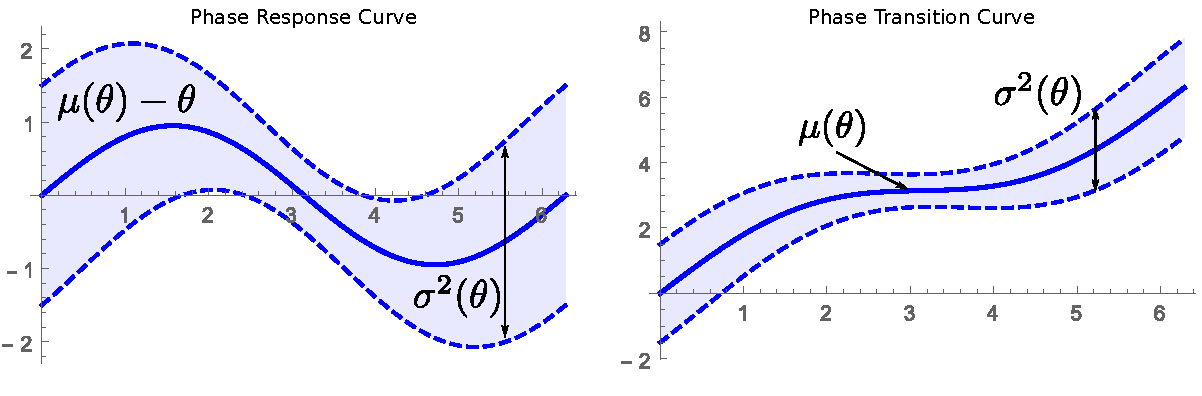
\includegraphics[width=\textwidth]{chap7/figures/prd.pdf}
  \titlecaption{Definition of the phase response distribution}{Inherent stochasticity in the response of a population of oscillators to stimulus could be captured by allowing a phase-dependent variance to be included in the phase response.}
  \label{fig:prd-def}
\end{figure}

A theoretical treatment of the phase response distribution might start with by the phase transition curve as mapping each initial phase to a distribution of perturbed phases $g(\theta_i) = {\cal WN}(\mu(\theta_i), \sigma^2(\theta_i); \theta_f)$.
A schematic of this is shown in \fref{fig:prd-def}.
The phase-transition function $g$ can therefore be imagined as a two-dimensional probability density function, in which $g(x, y)$ represents the probability of an oscillator with initial phase $x$ being transformed to a final phase $y$.
We will call this a phase transition surface, which is useful in calculating the oscillator probabilities following perturbation.

\begin{figure}[h!]
  \centering
  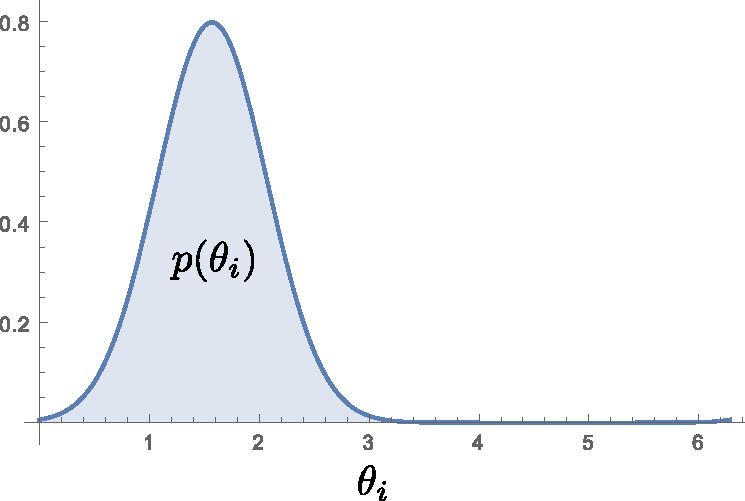
\includegraphics[width=0.5\textwidth]{chap7/figures/p.pdf}
  \titlecaption{Example probability density function for an initial population of oscillators}{Taken from a wrapped normal distribution with $\mu = \nicefrac{\pi}{2}$ and $\sigma^2 = 0.5$.}
  \label{fig:p}
\end{figure}

As an example, we take an initial phase population $p(\theta_i) = {\cal WN}(\nicefrac{\pi}{2}, 0.5)$ as shown in \fref{fig:p}.
In order to find the weighted probability of an oscillator at each initial phase $\theta_i$ being mapped to a final phase $\theta_f$, we multiply the initial population $p(\theta_i)$ by the phase transition surface $g(\theta_i, \theta_f)$ to find the weighted phase transition surface, as shown in \fref{fig:g}.

\begin{figure}[tbp]
  \centering
  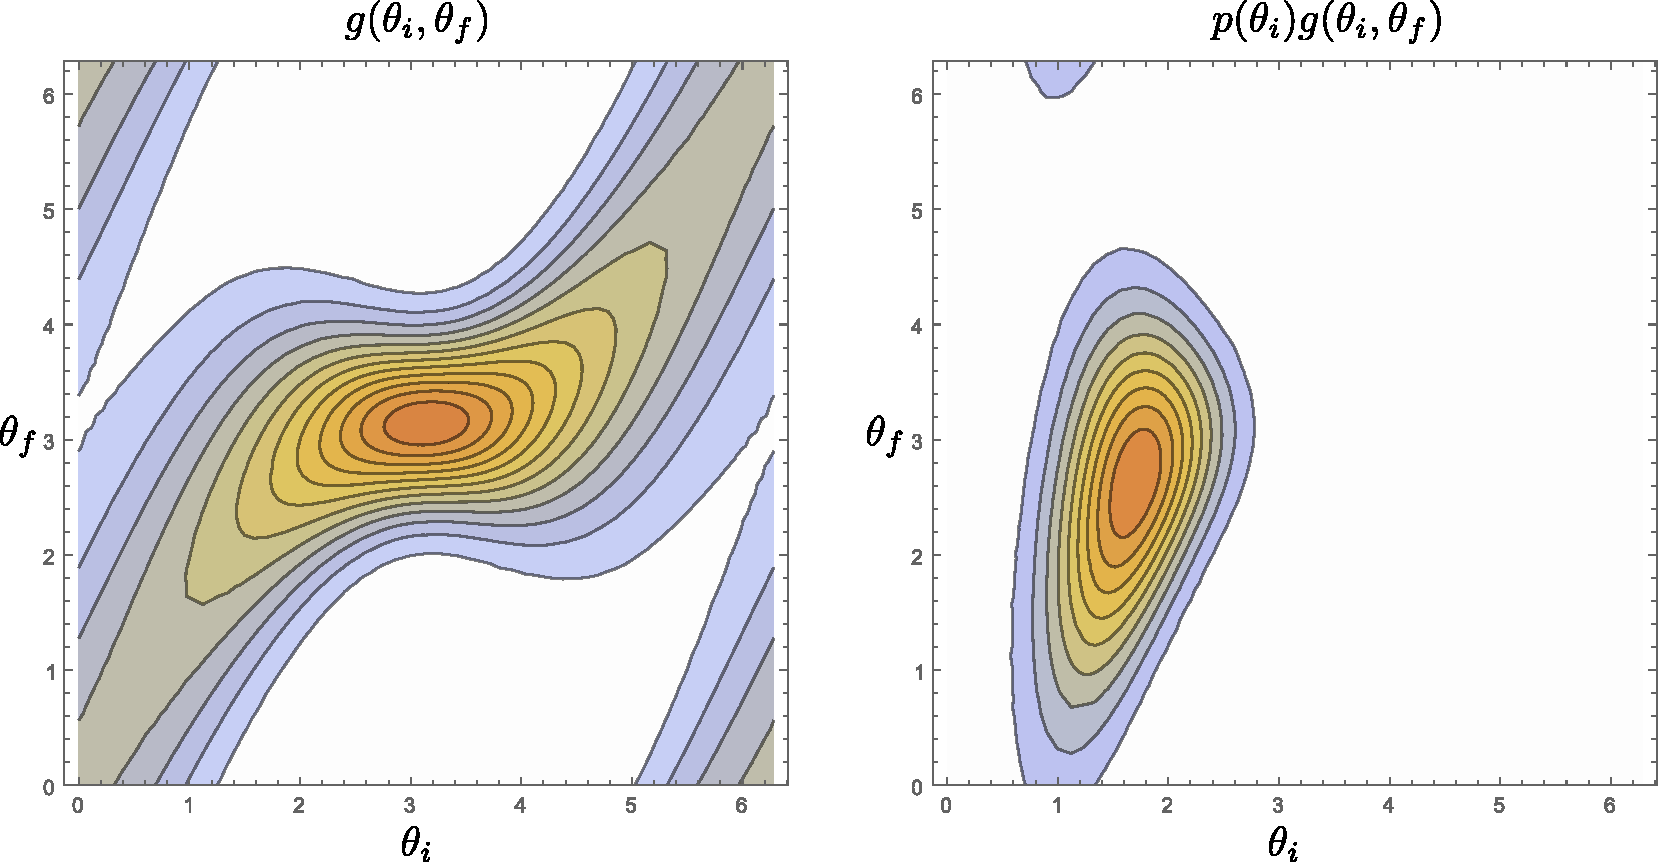
\includegraphics[width=\textwidth]{chap7/figures/g.pdf}
  \titlecaption{Phase transition surfaces}{The phase transition surface $g(\theta_i, \theta_f)$ and weighted phase transition surface $p(\theta_i) g(\theta_i, \theta_f)$. From the weighted phase transition surface, integrating in the vertical direction (marginal with respect to $\theta_i$) returns the phase probability density prior to perturbation ($p(\theta_i)$). Integrating in the horizontal direction returns the perturbed phase probability (denoted $\hat{p}(\theta_f)$ in \fref{chap:arc}).}
  \label{fig:g}
\end{figure}

From the weighted phase transition surface, finding the marginal distribution with respect to $\theta_i$ is relatively straightforward, and returns the initial phase density prior to perturbation:
\begin{align*}
  \int_0^{2\pi} p(\theta_i) g(\theta_i, \theta_f) \; d\theta_f &= p(\theta_i) \int_0^{2\pi} {\cal WN}(\mu(\theta_i), \sigma^2(\theta_i); \theta_f) \; d\theta_f \\
  &= p(\theta_i),
\end{align*}
since by definition the area under any wrapped normal distribution from $(0, 2\pi)$ is~$1$.

Finding the marginal distribution with respect to $\theta_f$, however, is considerably more difficult.
It can certainly be obtained numerically, as demonstrated in \fref{fig:phat7}.
The concept of phase response distributions has profound implications for entrainment and synchrony.
For instance, in a traditional phase-only model with a phase response curve, oscillators will synchronize at the fixed points defined where the PRC crosses 0 with a negative slope.
With a sufficiently small variance in the phase response distribution at a fixed point, relatively good entrainment will likely still be possible.
However, for a critical level of variance, it will likely be the case that entrainment to a given signal is no longer possible.

\begin{figure}[tbp]
  \centering
  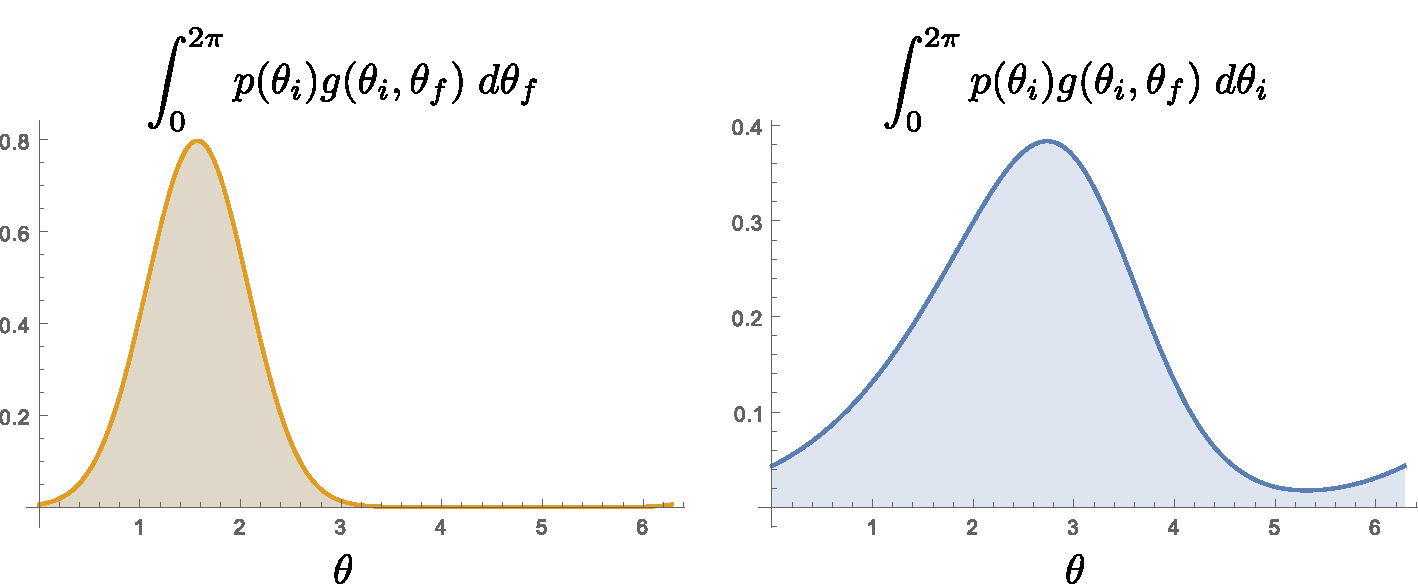
\includegraphics[width=0.9\textwidth]{chap7/figures/phat.pdf}
  \titlecaption{Marginal distributions of the weighted phase transition surface}{Calculating the marginal distributions of the weighted phase transition surface numerically. The marginal with respect to the final phase (left) returns the phase probability density prior to perturbation. The marginal with respect to the initial phase (right) returns the probability density after perturbation.}
  \label{fig:phat7}
\end{figure}

Finding an analytical solution to
\[
  \int_0^{2\pi} p(\theta_i) g(\theta_i, \theta_f) \; d\theta_i,
\]
possibly by using a series expansion of the mean and variance of the phase response distribution, would allow the relationship between the variance and derivative of the PRD at the fixed points to be determined.
Even if an analytical solution was not possible, a numerical investigation into the effect of noise in entraining signals.

\subsubsection{Quantifying phase response distributions}

In order for the above analysis to be applicable to experimental systems, we must also develop a suitable method for determining the phase response distribution from single-cell data.
This turns out to be a surprisingly difficult proposition, since many forms of error combine to reduce our ability to measure the mean and variance of the phase response.
Specifically, localizing a point on the phase response distribution from single-cell data introduces error in both the x-axis (phase before the pulse) as well as the y-axis (phase after the pulse).
Since the phase of any given cell is free to wander in a Brownian-type fashion, errors in both directions can be quite high.

One method for measuring the instantaneous phase of a nonstationary signal is the continuous wavelet transform, described in \fref{sec:cwt}.
Another uses the Hilbert transform, which produces an analytic representation of the initial signal in the complex plane.
The phase of the signal can then be obtained from the argument of the Hilbert transform, and used with a weighted linear regression to find an estimate of the phase just before and after perturbation.

To demonstrate such a method on {\itshape in silico} data, \fref{mod:hirota} was simulated stochastically at a range of different volumes.
Perturbations were applied at phases distributed across $(0, 2\pi)$, which consisted of $28\%$ reduction in the $vdp$ parameter (Per {\itshape mRNA} degradation) for $6.4$ hrs.
Control trajectories were simulated in the same fashion, but did not receive the pulse.
An example plot of the control and reference trajectories for are shown in \fref{fig:examplets}, showing the period and amplitude variability due to stochastic noise.

\begin{figure}[tbp]
  \centering
  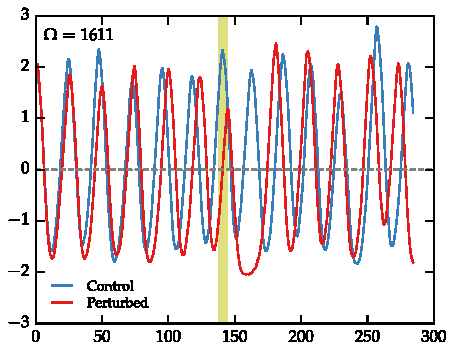
\includegraphics[width=0.6\textwidth]{chap7/figures/ts_example.pdf}
  \titlecaption{Example time-series measurements of noisy oscillators undergoing a phase response}{Simulated bioluminescence traces demonstrate the effect of a perturbation which induces a phase change. A control trajectory (blue) does not receive the pulse, but its phase wanders in time due to stochastic fluctuations. The perturbed trajectory (red) undergoes a transient change in amplitude due to the perturbation before settling back to the noisy limit cycle.}
  \label{fig:examplets}
\end{figure}

Example phase response distributions are shown for two volumes, $\Omega = 4897$, and $\Omega = 530$, in \fref{fig:measuredprds}.
Measurement errors seem to dominate the phase response distributions, such that even with $100$ data points it would likely be difficult to ascribe statistical significance to phase-dependent variance in the PRD.
Regardless, there may be ways of improving this quantification, and estimating the significance of any trends via Bayesian regression.
Errors in measuring $\theta_i$ and $\theta_f$ could be estimated from the combined variance of the control samples.

\begin{figure}[tbp]
  \centering
  \begin{subfigure}{0.475\textwidth}
    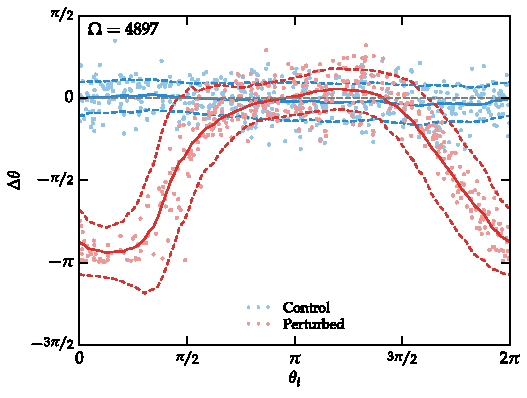
\includegraphics[width=\textwidth]{chap7/figures/4897.pdf}
    \caption{$\Omega = 4897$}
  \end{subfigure}
  \begin{subfigure}{0.475\textwidth}
    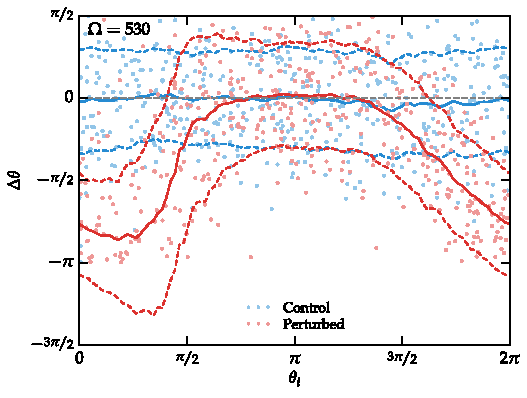
\includegraphics[width=\textwidth]{chap7/figures/530.pdf}
    \caption{$\Omega = 530$}
  \end{subfigure}
  \titlecaption{Measured phase response distributions}{Phase response distributions as determined for a case with low noise {\bfseries (a)} and high noise {\bfseries (b)}. Means and standard deviations (solid and dotted lines, respectively) are calculated from a moving window. In both cases measurement errors, as noticed by error in the control trajectory, will likely make the determination of phase-dependent changes in variance difficult.}
  \label{fig:measuredprds}
\end{figure}

\section{Improving identifiability of circadian models by minimizing energy usage}

In \fref{chap:id}, we describe a means of fitting optimal model parameters repeatedly to bootstrapped experimental data.
In using such a method, it became apparent that there were often structural identifiability issues in many circadian models, specifically with regard to protein turnover rate.
For example, it was often possible to capture a similar sinusoidal profile both with low degradation and low production rates, as well as high production and high degradation rates.
In techniques such as metabolic flux analysis, a large number of unknowns are optimized by assuming an organism has evolved towards some metabolic goal: for instance optimal growth or minimum energy consumption.
Such an approach might also be useful in optimizing circadian models, since actual genetic circuits would likely not use unrealistically high protein turnover rates.
By assigning an energy cost to the production of each molecule in the reaction network, the overall ``cost'' of running the model could be evaluated and minimized alongside the deviation from measured data.
A parameter to determine the relative weight of each term would be required, which could be tuned to improve model identifiability while maintaining close fits to experimental data.

\section{Conclusion}

While many of the research ideas expressed in this chapter seem like promising areas of research, there was sadly not enough time during my PhD to address all open ends.
Some projects, such as those described in \fref{sec:chida} and \fref{sec:prd}, were not pursued due to a lack of experimental tractability.
There is no reason to suspect that these limitations will always be the case, however, and therefore they may prove more fruitful in the future.

In general, circadian rhythms serve as an worthwhile example of the strides that can be taken between experimental and computational investigators.
Because the overlap in shared skills is often very little, it can be difficult for computational researchers to judge the quality of experimental work; just as it can be difficult for experimentalists to judge the methodology and reliability of mathematical models.
Collaborations are therefore essential not only in generating new data, but also in mutually understanding results in each sub-field.



